\chapter{Relation mellem designklasser} \label{bilagA}

\begin{figure} [H]
\centering
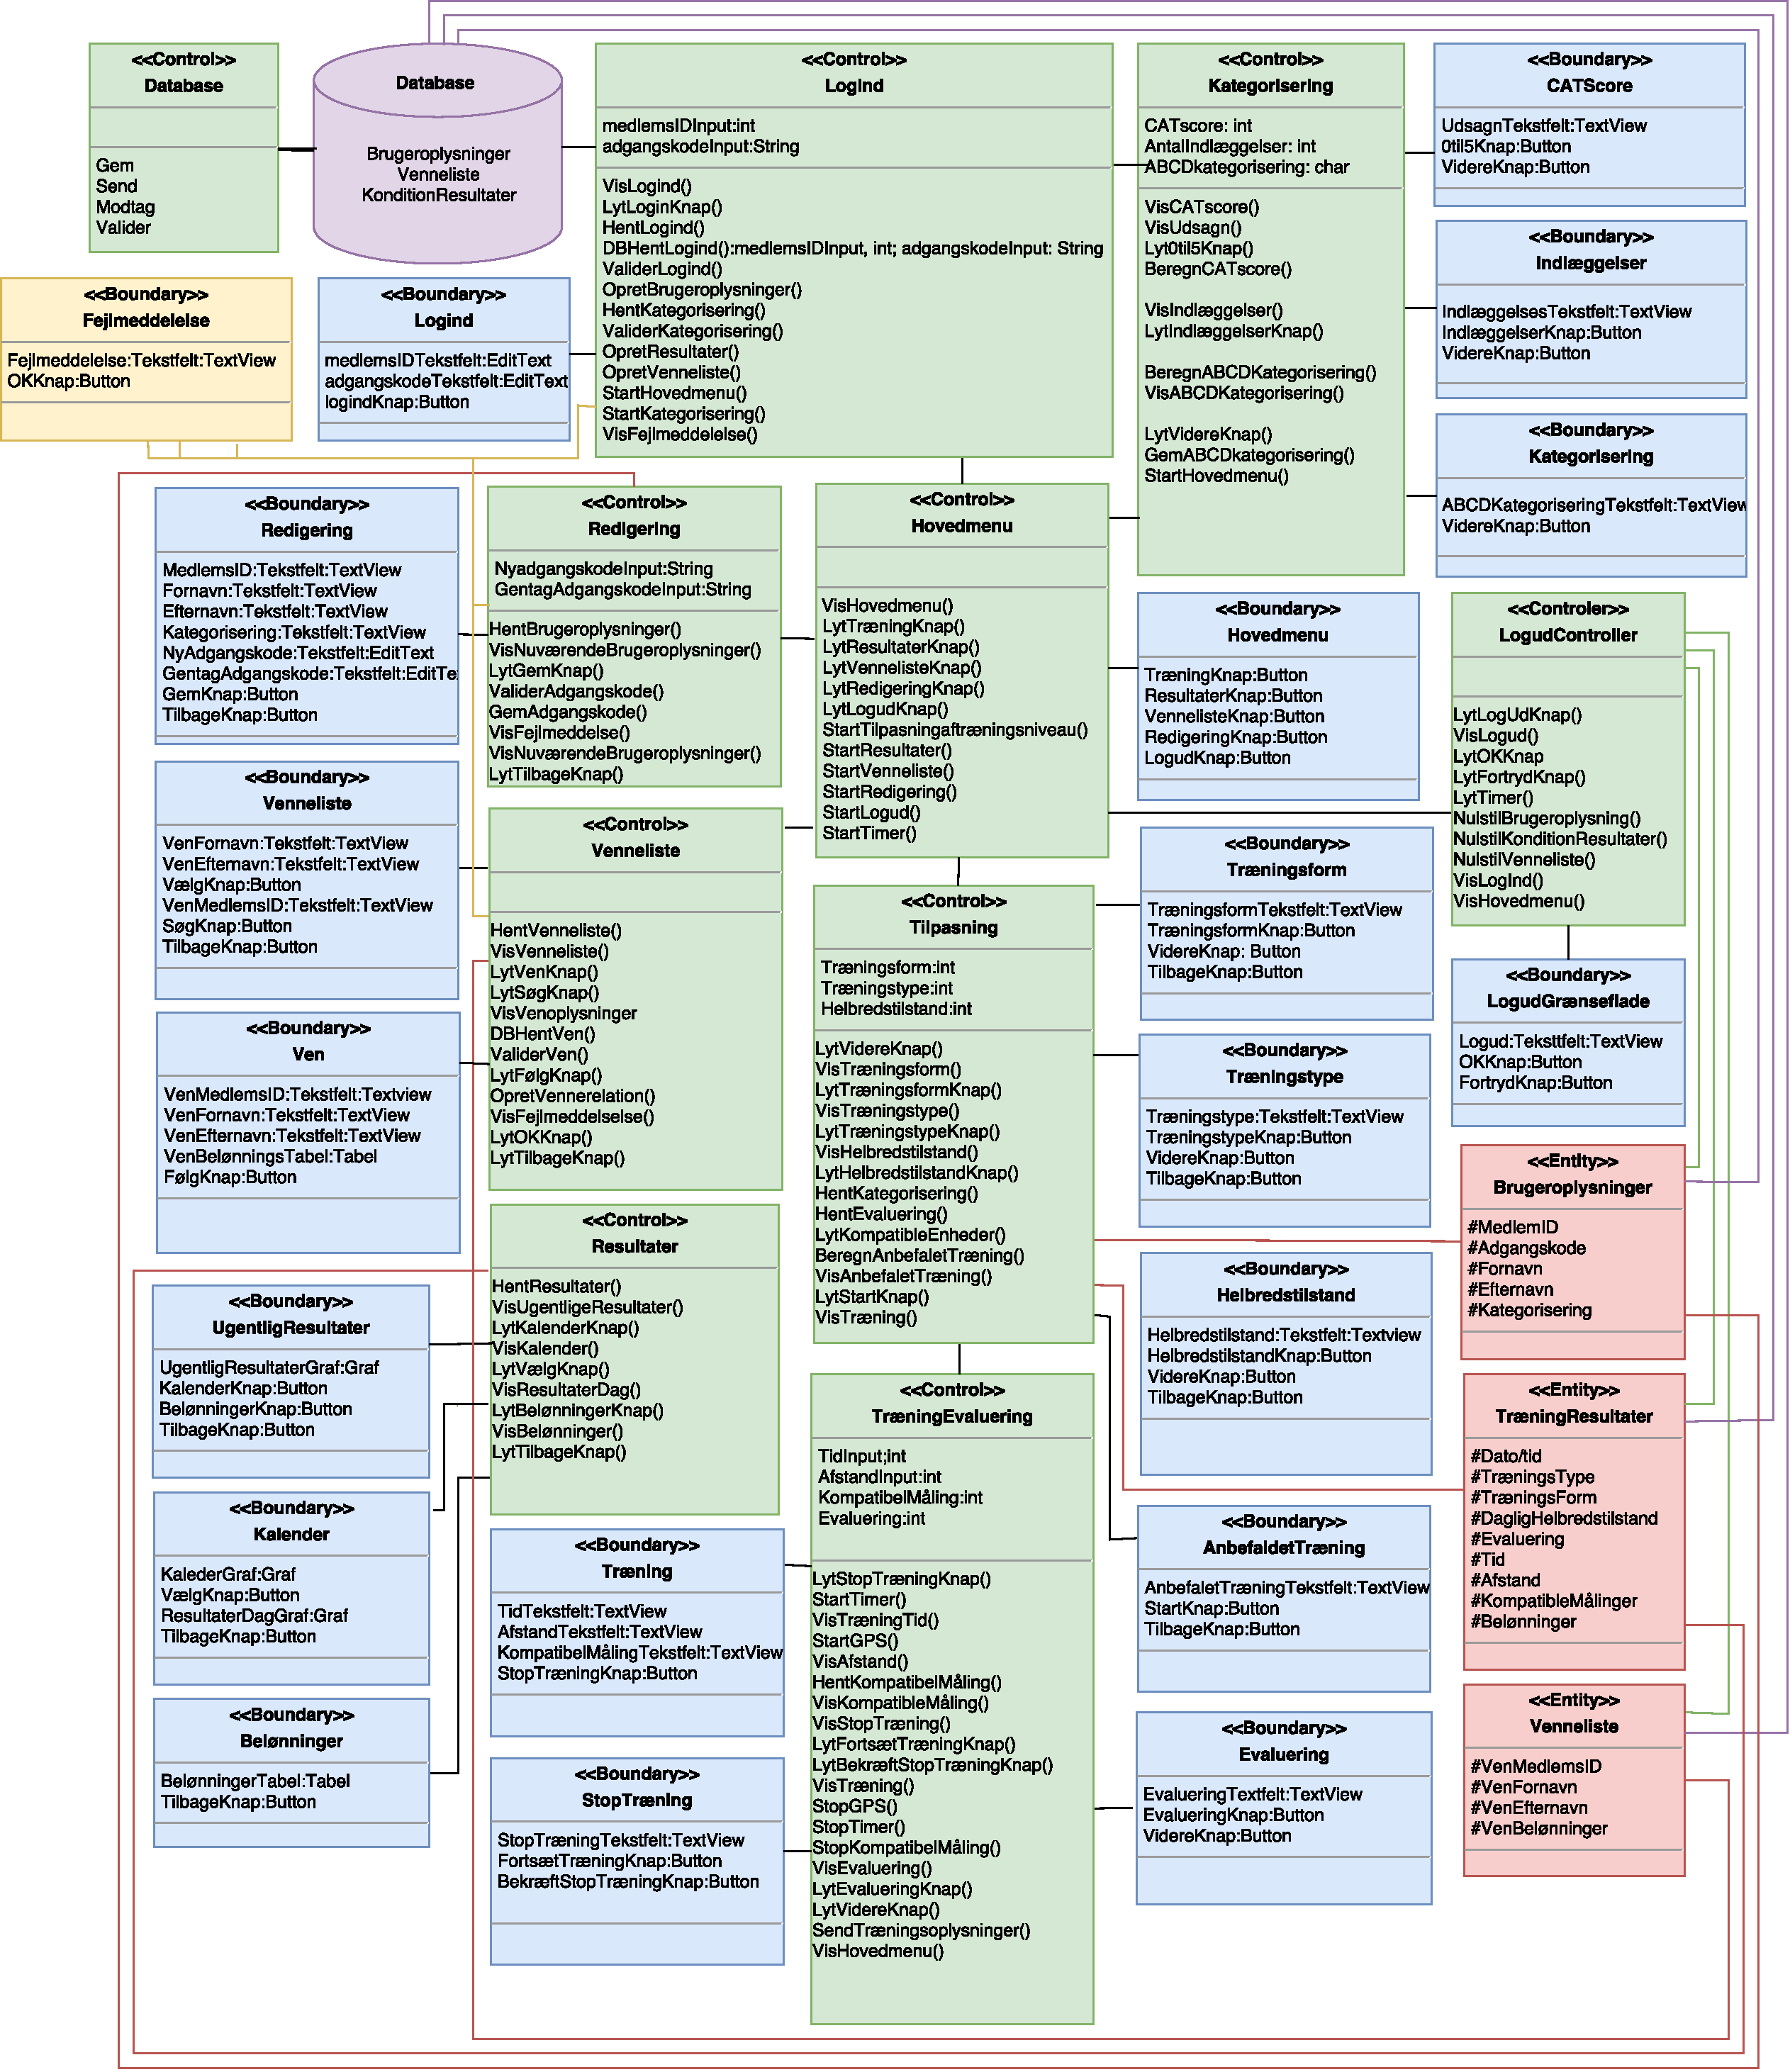
\includegraphics[width=0.85\textwidth]{figures/MVC/Designklasse}
\caption{Relationer mellem designklasser. Modelklasser er røde, viewklasser er blå, controllerklasser er grønne og Database samt databasecontroller er lilla. Indgår modellen Brugeroplysninger i en controller er disse markeret med en bordeaux kant. Er modellen KonditionResultater benyttet i en controller er dette markeret med en rød kant. Controllere tilknyttet til Databasen er markeret med lilla. }
\label{fig:Designklasser}
\end{figure}